%----------------------------------------------------------------------------------------
%	PACKAGES AND DOCUMENT CONFIGURATIONS
%----------------------------------------------------------------------------------------

\documentclass[a4paper, 12pt]{article}
\usepackage[version=4]{mhchem} % Package for chemical equation typesetting
\usepackage{siunitx} % Provides the \SI{}{} and \si{} command for typesetting SI units
\usepackage{amsmath} % Required for some math elements 
\usepackage{times} % Uncomment to use the Times New Roman font
\usepackage[backend=biber, bibencoding=utf-8, style=chem-acs, citestyle=chem-acs, sorting=none]{biblatex}
\setlength{\parskip}{1em}
\addbibresource{references.bib}
\usepackage{geometry}
\geometry{margin=1in}
\usepackage{textcomp}
\usepackage{graphicx}
\graphicspath{ {./images/} }

%----------------------------------------------------------------------------------------
%	DOCUMENT INFORMATION
%----------------------------------------------------------------------------------------

\title{Analysis and Quantification of 2,2',4,4'-Tetrabromodiphenyl Ether using Gas Chromatography - Electron Ionization, Coupled with a Low-Resolution Mass Spectrometry in the Selected Ion Monitoring \\ CHEM 4303 \\ Analytical Separations} % Title

\author{Robby \textsc{Renz}} % Author name

\date{\today} % Date for the report

\begin{document}

\maketitle % Insert the title, author and date

\begin{center}
	\begin{tabular}{l r}
		Date Performed: & November 13, 2018 \\ % Date the experiment was performed
		Date Completed: & November 27, 2018 \\
		Partner: & Jaya Roe \\ % Partner name
		Lab Instructor: & Kevin Stroski % Instructor/supervisor
	\end{tabular}
\end{center}

%----------------------------------------------------------------------------------------
%	SECTION 1
%----------------------------------------------------------------------------------------

\begin{abstract}
	Gas chromatography - electron ionization mass spectrometry in the selected ion monitoring (GC/EI-MS-SIM) was used to detect and quantify the amount of BDE-47 in fish oil. Initially, the mass spectrum and total ion chromatogram was obtained for the analyte in question, BDE-47, the internal standard PBB-77 and the recovery standard `2-\ce{HCH}. Afterwards, 2 samples of fish oil was prepared using solid-phase extraction. Finally, the fish samples, blanks, BDE-47, PBB-77 and `2-\ce{HCH} underwent GC/EI-MS-SIM analysis, in which the ions being monitored were at a m/z of 326 and 486 for BDE-47, 470 and 310 for PBB-77, and 181 and 219 for `2-\ce{HCH}. Through calculations, it was realized that the average concentration of BDE-47 in the first sample of fish oil was  \SI{1.47e-5}{\ug/g} \num{+-1.07}\%, while the second sample of fish oil had a BDE-47 concentration of \SI{1.66e-5}{\ug/g} \num{+-13.75}\%.
\end{abstract}
\newpage

%----------------------------------------------------------------------------------------
%	SECTION 2
%----------------------------------------------------------------------------------------

\section{Introduction}
Gas chromatography (GC) is a separation technique that analyzes volatile compounds \cite{vitha_chromatography:_2017}. Consequently, this analysis can lead a lot of useful situations such as the determination of the purity of a compound or even quantifying individual components in mixtures \cite{vitha_chromatography:_2017}. In GC, the analyte is volatilized and carried through the column by the mobile phase, often called the carrier gas \cite{harris}. This carrier gas can either be \ce{He} or \ce{H2} \cite{harris}. These gases are often chosen as the carrier gas as they are chemically inert and would therefore not react with the analytes \cite{vitha_chromatography:_2017}.

Polybrominated diphenyl ethers (PBDEs) are a class of halogenated compounds that are commonly used as flame retardants \cite{bjorklund_mass_2003}. These compounds are an environmental health hazard as they have the potential to accumulate in the food chain \cite{thomsen_comparing_2002}. In addition, 2,2',4,4'-Tetrabromodiphenyl ether, also known as BDE-47 \cite{rat}, is a PBDE congener, and has been found to cause neurotoxic effects in adults \cite{thomsen_comparing_2002}. Commonly used detection techniques for PBDEs are high-resolution mass spectrometry and low-resolution mass spectrometry (LRMS) \cite{bjorklund_mass_2003}.

LRMS is commonly done with selected ion monitoring (SIM) \cite{bjorklund_mass_2003}. SIM increases the selectivity of mass spectrometry for analytes and reduces its response to everything else \cite{harris}. It does this by setting the mass spectrometer to detect just one or even a few m/z values \cite{harris}. One of the advantages of SIM is that the signal-to-noise ratio greatly increases as the mass spectrometer spends its entire analysis time measuring that particular ion, or a couple of ions \cite{harris}.

Internal standards are used for a number of reasons, such as when sample loss is expected during the sample preparation step, or when the response of the quantity of sample detected differs at each analysis \cite{harris}. Essentially, an internal standard is a known quantity of a compound that differs from the analyte, and is added to the mixture containing the analyte to be detected \cite{harris}. 

An injection mode of splitless rather than a split is used when attempting to analyze trace chemicals \cite{harris}. Furthermore, a splitless injection mode minimizes solvent tailing by opening the split vent after around \SI{1}{min} so that the any remaining sample in the injection port can be purged \cite{vitha_chromatography:_2017}.

The main objective of this entire experiment is to detect as well as quantify BDE-47 in a sample of fish oil. This is accomplished by making a method that utilizes a SIM.

%----------------------------------------------------------------------------------------
%	SECTION 3
%----------------------------------------------------------------------------------------

\section{Chemicals, Methods and Instrumentation}

\subsection{Chemicals}
In the first week, BDE-47, PBB-77 and `2-\ce{HCH}, all of each were at a concentration of \SI{50}{\mu{}g/mL} in isooctane, were used as standard solutions. In the second week, fish oil (Exact Norwegian Cod Liver Oil), dichloromethane (emd, Lot 5Q160, CAS: 75-09-2) and PBB-77, at a concentration of \SI{10}{\mu{}g/mL} in isooctane, were used as chemicals. Finally, in the last week, BDE-47, PBB-77 and `2-\ce{HCH}, each at a concentration of \SI{10}{\mu{}g/mL} in isooctane, were used. Throughout the entirety of the experiment, hexane (Caledon Laboratory Chemicals, CAS no. 110-54-3, LOT: 89001) and isooctane (OmniSolv, CAS: 540-84-1, LOT: 52054) were used.

\subsection{Instrumentation}
The separation and analysis of the entire experiment was performed on an Agilent 7890A GC, coupled with a 5975C inert XL EI/CI MSD with a triple axis detector. The dimensions of the column used was $30m \times 0.250mm \times 0.25\mu{}m$, by Agilent Technologies. The stationary phase was (5\%-Phenyl)-methylpolysiloxane. Each analysis was performed with the injection mode at splitless, with \ce{He} as the carrier gas, and the flow rate was set at \SI{1}{mL/min}. The injection mode used for each analysis was splitless, and the injection volume was \SI{2}{\mu{}L} for each analysis.

\subsection{Methods}
In the first week of the experiment, a (normalized) full scan spectrum was obtained for BDE-47, PBB-77 and `2-\ce{HCH}. The upper limit of the scan range was set to 30 \si{\amu} more than the molecular weight of the respective analyte that was being analyzed. For each analysis, the oven temperature was initially set to \SI{100}{\degreeCelsius} for \SI{5}{min}, then it was increased to \SI{280}{\degreeCelsius} at a rate of \SI{10}{\degreeCelsius/min}, and it was held at that temperature for \SI{7}{min}. Furthermore, the temperature of the splitless injection port was set to \SI{260}{\degreeCelsius}, the electron energy was set to \SI{70}{eV}, and the temperature of the GC-MSD interface was fixed at a temperature of \SI{280}{\degreeCelsius}.

In the second week of the experiment, two samples of fish oil were prepared by adding \SI{2}{\mu{}g/mL} of PBB-77 as the internal standard to the sample, and then having it undergo solid-phase extraction in order to extract lipids. Afterwards, the majority of the solvent was then removed from the sample through rotary evaporation.

In the last week of the experiment, a calibration solution was produced by adding each of BDE-47 and PBB-77, at a volume of \SI{10}{\mu{}L}, to a \SI{0.5}{mL} of isooctane contained in an auto sampler vial, and it was diluted all the way to \SI{1.0}{mL} with the solvent. \SI{50}{\mu{}L} of `2-\ce{HCH} was added to the calibration solution, while \SI{10}{\mu{}L} was added to the fish samples that was prepared last week. Finally, the GC-MS was set to scan only two ions per analyte, the parameters that was selected is shown in table \ref{tab-para}. Refer to table ref to see which 2 ions was monitored.

%----------------------------------------------------------------------------------------
%	SECTION 4
%----------------------------------------------------------------------------------------

\section{Results and Discussion}

\subsection{Results}
All of the GC/EI MS chromatograms are located in the `Chrmoatograms' subsection in the `Appendix' section, and all them are appropriately labelled.

Table \ref{tab-para} shows the parameters that was set in the GC/EI-MS and the mass of the ions that was monitored.

\begin{table}[h!]
	\centering
	\caption{Selected Ion Monitoring Parameters}
	\hfill \\
	\begin{tabular}{|c|c|c|}
		\hline
		Compound & Ions monitored (m/z) & Time window (min) \\
		\hline
		`2-\ce{HCH} & 181, 219 & 0.5 - 19 \\
		\hline
		BDE-47 & 326, 486 & 19 - 22.5 \\
		\hline
		PBB-77 & 470, 310 & 22.5 - 24 \\
		\hline
	\end{tabular}
	\label{tab-para}
\end{table}

Table \ref{tab-mass} tabulates the molecular weight of BDE-47, PBB-77, and `2-\ce{HCH}.

\begin{table}[h!]
	\centering
	\caption{Molecular weight of BDE-47, PBB-77 and `2-HCH}
	\hfill \\
	\begin{tabular}{|c|c|}
		\hline
		Compound & Molecular weight (\si{\amu}) \\
		\hline
		BDE-47 & 486 \\
		\hline
		PBB-77 & 470 \\
		\hline
		`2-\ce{HCH} & 291 \\
		\hline
	\end{tabular}
	\label{tab-mass}
\end{table}

Table \ref{tab-fish} shows mass of fish oil that was weighed out for this experiment.

\begin{table}[h!]
	\centering
	\caption{Mass of fish oil weighed out}
	\hfill \\
	\begin{tabular}{|c|c|}
		\hline
		Sample number & Mass (\si{\gram}) \\
		\hline
		1 & 1.1234 \\
		\hline
		2 & 0.9062 \\
		\hline
	\end{tabular}
	\label{tab-fish}
\end{table}

Table \ref{tab-pre-rrf} tabulates the volume, concentration and mass of BDE-47, PBB-77, and `2-\ce{HCH} that was added into the calibration solution, while table \ref{tab-rrf} shows the response and relative response factors of the aforementioned analytes to the internal standard, which was PBB-77, in the calibration solutions.

\begin{table}[h!]
	\centering
	\caption{Table of data showing the volume and concentration of each analyte in the calibration solution}
	\hfill \\
	\begin{tabular}{|c|c|c|c|c|c|c|}
		\cline{1-5}
		Component      & Volume/\si{mL}   & Concentration(\si{\mu{}g/mL}) & Mass/\si{\mu{}g}      & Area    \\ \cline{1-5}
		BDE-47         & 0.01             & 0.0952                        & \num{9.52e-04}        & 367089  \\ \cline{1-5}
		PBB-77         & 0.01             & 0.0952                        & \num{9.52e-04}        & 230205  \\ \cline{1-5}
		`2-\ce{HCH}    & 0.05             & 0.476                         & \num{2.38e-02}        & 260358  \\ \cline{1-5}
	\end{tabular}
	\label{tab-pre-rrf}
\end{table}

\begin{table}[h!]
	\centering
	\caption{Table of data showing the response and relative response factors of each analyte to the internal standard (PBB-77) in the calibration solution}
	\hfill \\
	\begin{tabular}{|c|c|c|c|c|c|c|}
		\cline{1-5}
		Component      & Mass/\si{\mu{}g}        & Area          & Response factor/\si{\mu{}u}       & Relative Response Factor       \\ \cline{1-5}
		BDE-47         & \num{9.52e-04}          & 367089        & \num{2.59e-09}                    & \num{6.27e-01}                 \\ \cline{1-5}
		PBB-77         & \num{9.52e-04}          & 230205        & \num{4.14e-09}                    & \num{1.00e+00}                 \\ \cline{1-5}
		`2-\ce{HCH}    & \num{2.38e-02}          & 260358        & \num{9.14e-08}                    & \num{2.21e+01}                 \\ \cline{1-5}
	\end{tabular}
	\label{tab-rrf}
\end{table}

Table \ref{tab-mass-of-bde} shows how much mass of BDE-47 was contained in each sample of fish.

\begin{table}[h!]
	\centering
	\caption{Table of data showing how much mass of BDE-47 is in each fish sample}
	\hfill \\
	\begin{tabular}{|c|c|c|c|}
		\hline
		Fish sample                & Area of BDE-47 & Area of PBB-77 & Mass of BDE-47 in sample/\si{\mu{}g}     \\ \cline{1-4}
		1 (first run)              & 13799          & 100528         & \num{1.64e-05}                           \\ \cline{1-4}
		1 (second run)             & 14383          & 103212         & \num{1.66e-05}                           \\ \cline{1-4}
		2 (first run)              & 12800          & 112480         & \num{1.36e-05}                           \\ \cline{1-4}
		2 (second run)             & 13938          & 100772         & \num{1.65e-05}                           \\ \cline{1-4}
	\end{tabular}
	\label{tab-mass-of-bde}
\end{table}

Table \ref{tab-areas} shows the mass of PBB-77 and `2-\ce{HCH} that was added to the calibration solution as well as areas of their respective peaks.

\begin{table}[h!]
	\centering
	\caption{Mass of PBB-77 and `2-\ce{HCH} that was added to the calibration solution}
	\hfill \\
	\begin{tabular}{|c|c|}
		\hline
		Mass of PBB-77 /\si{\mu{}g}      & Mass of ‘2-\ce{HCH}/\si{\mu{}g}    \\ \hline
	    \num{1.90e-04}                   & \num{4.76e-03}                     \\ \hline
	\end{tabular}
	\label{tab-areas}
\end{table}

Table \ref{tab-recovery} shows the recovery rate of the internal standard, PBB-77, in each fish sample.

\begin{table}[h!]
	\centering
	\caption{Recovery rate of PBB-77 in each fish sample}
	\hfill \\
	\begin{tabular}{|c|c|c|}
		\hline
		Fish sample        & Mass of PBB-77 recovered/\si{\mu{}g} & Actual Recovery Rate/\% \\ \hline
		1 (first run)      & \num{4.90e-05}                             & 25.72                   \\ \hline
		1 (second run)     & \num{4.99e-05}                             & 26.22                   \\ \hline
		2 (first run)      & \num{8.38e-05}                             & 44.04                   \\ \hline
		2 (second run)     & \num{7.60e-05}                             & 39.90                   \\ \hline
	\end{tabular}
	\label{tab-recovery}
\end{table}

Table \ref{tab-mean} shows the average concentration of BDE-47 in fish oil. The table also shows the relative standard deviation of the concentration as well.

\begin{table}[h!]
	\centering
	\caption{The mean, standard deviation, and relative standard deviation of BDE-47 in fish oil in both of the samples}
	\hfill \\
	\begin{tabular}{|c|c|c|c|}
		\hline
		Fish sample & Mean of BDE-47 in fish oil/(\si{\mu{}g/g}) & Std. Dev./(\si{\mu{}g/g}) & Relative Std. Dev./\% \\ \hline
		1           & \num{1.47e-05}                             & \num{1.57e-07}            & 1.07                  \\ \hline
		2           & \num{1.66e-05}                             & \num{2.28e-06}            & 13.75                 \\ \hline
	\end{tabular}
	\label{tab-mean}
\end{table}

Table \ref{tab-sn} shows the average signal-to-noise ratio of BDE-47 in the fish samples.

\begin{table}[h!]
	\centering
	\caption{Average signal-to-noise ratio of BDE-47 in the fish samples}
	\hfill \\
	\begin{tabular}{|c|c|}
		\hline
		Fish sample & Signal-to-Noise ratio    \\ \hline
		1           & 93.65                    \\ \hline
		2           & 7.27                     \\ \hline
	\end{tabular}
	\label{tab-sn}
\end{table}



\subsection{Discussion}
\setcounter{figure}{23}
The mass spectra for the compounds BDE-47, PBB-77 and `2-\ce{HCH} shown in figures 3,4 and 5 respectively. And the identification of its corresponding molecular ion (M+) is illustrated in figures 24, 25 and 26, except that they have an extra positive charge in the molecule. Note that the figures were taken from the website PubChem [The PubChem Project. https://pubchem.ncbi.nlm.nih.gov/ (accessed Dec 11, 2018)].

\begin{figure}[h!]
	\centering
	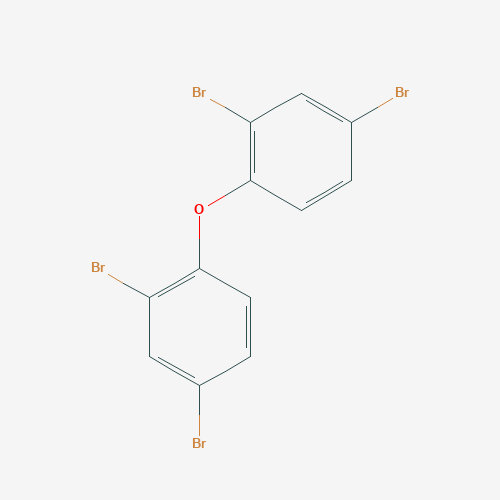
\includegraphics[width=1\textwidth]{bde-47.png}
	\caption{Molecular structure of BDE-47}
	\label{fig-bde}
\end{figure}

\begin{figure}[h!]
	\centering
	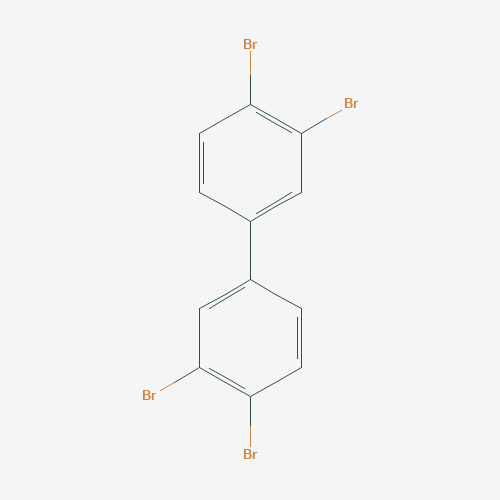
\includegraphics[width=1\textwidth]{pbb-77.png}
	\caption{Molecular structure of PBB-77}
	\label{fig-pbb}
\end{figure}

\begin{figure}[h!]
	\centering
	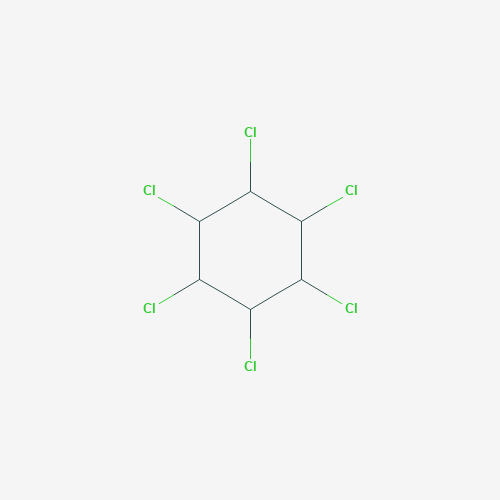
\includegraphics[width=1\textwidth]{lindane.png}
	\caption{Molecular structure of `2-\ce{HCH}}
	\label{fig-lindane}
\end{figure}

As it can be seen in figures 

%----------------------------------------------------------------------------------------
%	SECTION 5 (BIBLIOGRAPHY)
%----------------------------------------------------------------------------------------

\section{References}
\printbibliography

%----------------------------------------------------------------------------------------
%	SECTION 6
%----------------------------------------------------------------------------------------

\section{Appendix}

\subsection{Calculations}


\begin{description}

	\item[Calculating the final concentration of BDE-47 in the calibration solution] \hfill \\
		\begin{equation} \label{equ-conc}
			\begin{split}
				\textit{initial concentration} \times \frac{\textit{initial volume}}{\textit{final volume}} & = \textit{final concentration} \\
				10 \si{\mu{}g/mL} \times \frac{0.01\si{mL}}{1.05\si{mL}} & = 0.0952 \si{\mu{}g/mL}
			\end{split}
		\end{equation}
		Equation \ref{equ-conc} was taken from \cite{harris}.

	\item[Calculating the relative response factor of BDE-47] \hfill \\
		\begin{gather*} \label{equ-rrf}
				\textit{Mass of BDE-47 in the calibration solution} = \textit{volume} \times \textit{concentration} \\
				0.01\si{mL} \times 0.0952 \si{\mu{}g/mL} = \SI{9.52e-4}{\mu{}g} \\
				\textit{Response Factor} = \frac{\textit{Mass}}{\textit{area}} \\
				\frac{\SI{9.52e-04}{\mu{}g}}{367089} = \SI{2.59e-09}{\mu{}g} \\
				\textit{Relative response factor} = \frac{\textit{Response factor}_{BDE-47}}{\textit{Response factor}_{PBB-77}} \\
				\frac{\num{2.59e-9}}{\num{4.14e-09}} = \num{6.27e-1}
		\end{gather*}

	\item[Actual recovery rate of internal standard, PBB-77, for the first run of fish sample 1] \hfill \\
		\begin{gather*}
			\textit{Actual Recovery Rate} = \frac{\textit{Mass}_{IS_{recovered}}}{\textit{Mass}_{IS_{added}}} \\
			\frac{\num{4.90e-5}}{\num{2.21e1}} = 25.72\%
		\end{gather*}

\end{description}


\subsection{Chromatograms}
There are 23 figures of GC/EI chromatograms.

%----------------------------------------------------------------------------------------


\end{document}
